\scanpage{29}

$\Gamma=\mathbb G$

\margin{$M\times B'\qquad\operatorname{Ext}(B',DM)$

$\deleted{\operatorname{Hom}(B',\operatorname{Ext}(\unsure{M},\unsure{\mathbb G_m}))}=0$}

\diagram{\begin{tikzcd}[ampersand replacement=\&, row sep=small,column sep=small]
B \& B'\\
M \arrow[u,"i"] \& M' \arrow[u,"i'"']
\end{tikzcd}}
\quad \unsure{une} biext.\inserted{$\mathcal E$} sous $\mathbb G_m$

\diagram{\begin{tikzcd}[ampersand replacement=\&, column sep=small]
B' \arrow[r,"\alpha'"] \& \underline{\operatorname{Ext}}(B,G_m) \arrow[r,no head] \& \underline{\operatorname{Ext}}(M\ G_m)
\end{tikzcd}}
nul\quad p.c. $\operatorname{Hom}(B',\underline{\operatorname{Ext}}(M,\overset{\substack{0\\\Vert}}{G_m}\unsure{)}$

\diagram{\begin{tikzcd}[ampersand replacement=\&, column sep=small]
B \arrow[r,no head,"\alpha"] \& \underline{\operatorname{Ext}}(B',G_m) \arrow[r,no head] \& \underline{\operatorname{Ext}}(M',G_m)
\end{tikzcd}}
nul\quad p.ex $\operatorname{Hom}(B,\underline{\operatorname{Ext}}(M',\underset{\substack{\Vert\\0}}{G_m}\unsure{)}$

d'où extensions,

\diagram{\begin{tikzcd}[ampersand replacement=\&, column sep=small,row sep=tiny]
\bullet \arrow[r,no head] \& DM \arrow[r,no head,"j'"] \arrow[d,equal] \& G' \arrow[r,no head,"p'"] \& B' \arrow[r] \& 0\\
 \& T' \& \& \&
\end{tikzcd}}

\margin{\par\noindent\rule{0.8\linewidth}{0.3pt}\par
$\mathcal E_{M,G'}$ est canoniq\textsuperscript{t}\par splitté par $\rho$
\par\noindent\rule{0.8\linewidth}{0.3pt}\par}

\diagram{\begin{tikzcd}[ampersand replacement=\&, column sep=small,row sep=tiny]
0 \arrow[r,no head] \& DM' \arrow[r,no head,"j"] \arrow[d,equal] \& G \arrow[r,no head,"p"] \& B \arrow[r] \& 0\\
 \& T \& \& \&
\end{tikzcd}}

\margin{$\mathcal E_{G,M'}$ est can.\par splitté $\rho'$
\par\noindent\rule{0.8\linewidth}{0.3pt}\par}

\uline{\unsure{Exemp}} si \deleted{\illegible{1}} $\uline{\alpha'}$ \deleted{\illegible{1}} \inserted{\unsure{est}} un isom, \unsure{alors} $i'$ \unsure{rev\textsuperscript{t}|vers} : \unsure{à} \unsure{donner|donné}

\noindent un
\diagram{\begin{tikzcd}[ampersand replacement=\&,column sep=small]
i'\in\operatorname{Hom}(M',\underline{\operatorname{Ext}}(B,G_m))
\& \operatorname{Biext}(B,M';G_m) \arrow[l,"\sim"']
\& \inserted{\operatorname{Ext}(B,D(M'))} \arrow[l,"\sim"']
\end{tikzcd}}
\noindent\hfill\deleted{\unsure{réciproq\textsuperscript{t}}}\hspace{1.3em}
\begin{flushright}
\begin{minipage}[t]{0.47\linewidth}

\begin{tikzpicture}[baseline,overlay]
\draw (0,0.65) .. controls (0,0.25) and (0,0.15) .. (0.22,0.08);
\end{tikzpicture}\hspace{0.25cm}si $\underline{\unsure{\operatorname{Ext}}}(M',\underline{\operatorname{Hom}}(B,G_m))=0$

p.ex
\makebox[0pt][l]{\begin{tikzpicture}[baseline,overlay]\draw (2.59,.36) .. controls (1.75,.51) and (.35,.44) .. (-.03,.08) .. controls (-.16,-.13) and (.77,-.29) .. (1.64,-.24) .. controls (2.34,-.18) and (2.92,-.12) .. (2.78,.23);\end{tikzpicture}}$\underline{\operatorname{Hom}}(B,G_m)=0$
\end{minipage}\hfill
\begin{minipage}[t]{0.47\linewidth}

\begin{tikzpicture}[baseline,overlay]
\draw (0,0.65) .. controls (0,0.25) and (0,0.15) .. (0.22,0.08);
\end{tikzpicture}\hspace{0.25cm}si $\operatorname{Hom}(B,\underline{\operatorname{Ext}}(M',G_m))$

$=0$\quad p.ex.

\makebox[0pt][l]{
\begin{tikzpicture}[baseline,overlay]\draw (-.05,.28) .. controls (.13,.39) and (.24,.22) .. (.43,.31) .. controls (.85,.42) and (1.13,.30) .. (1.43,.34) .. controls (2.23,.42) and (2.57,.64) .. (2.76,.25) .. controls (3.12,-.21) and (2.22,-.47) .. (1.80,-.36) .. controls (1.21,-.51) and (.44,-.48) .. (.10,-.20) .. controls (.01,-.10) and (-.02,.03) .. (.02,.16);\end{tikzpicture}}$\underline{\operatorname{Ext}}(M',G_m)=0$
\end{minipage}
\end{flushright}

\unsure{aussi|ainsi} pour. \unsure{Donc} la donnée de $i'$ \unsure{équiv} : celle de l'ext. $G$. Et \unsure{réciproquement}

Considérons l'image inverse\makebox[0pt][l]{
\begin{tikzpicture}[baseline,overlay]\draw (.12,-.12) .. controls (-.28,.20) and (-.17,.70) .. (.25,.75) .. controls (.75,.92) and (1.10,.65) .. (1.14,.31) .. controls (1.20,.09) and (.48,-.12) .. (.27,-.29) .. controls (.16,-.39) and (.20,-.53) .. (.26,-.61);\end{tikzpicture}}\inserted{$\mathcal E_{\unsure{i'|i},i'}$}
de $\mathcal E$ sur $(M,M')$. Alors des \unsure{splittages|splittage}\inserted{$\rho_i$} de cette biextension correspondent aux hom $j$ de $M$ dans $G$ relevant $i$, \unsure{ou aux|ou à}\,$j'$ de $M'$ dans $G'$ relev. de $i'$.

\diagram{\begin{tikzcd}[ampersand replacement=\&, row sep=tiny,column sep=small]
M \arrow[r,no head] \& G \arrow[r,no head] \& B\\
M' \arrow[r,no head] \& G' \arrow[r,no head] \& B'
\end{tikzcd}}

\makebox[0pt][l]{\begin{tikzpicture}[baseline,overlay]\draw (.01,-.12) .. controls (-.18,.13) and (-.02,.40) .. (.49,.39) .. controls (.99,.39) and (1.34,.28) .. (1.36,.09) .. controls (1.40,-.10) and (.39,-.22) .. (.14,-.18);\end{tikzpicture}}\deleted{\unsure{dans le|sur $k$}}

\deleted{\unsure{Si}} \inserted{Deux \unsure{relèv\textsuperscript{ts}|relèvements}} $j$ et $j'$ \deleted{\unsure{se}} correspond ainsi

\deleted{\unsure{les|des} \unsure{conditions} splitt. $\sigma$ canonique \deleted{\illegible{1}} $\sigma$ de $\mathcal E_{G,M'}$ et un splitt. $\sigma$ canonique $\sigma'$ de $\mathcal E_{M,G'}$, ces \unsure{deux} splitt. $\sigma$ coïncident sur $M,M'$ \unsure{avec} le splittage \unsure{donné} $h$ de $\mathcal E_{M,M'}$.}

ssi les deux splittages de $\mathcal E_{M,M'}$\unsure{)|,} \unsure{les|l'un} \unsure{déduits|déduit} d'\unsure{une|eux} par du splittage $\rho$ de $\mathcal E_{M,G'}$ \unsure{et} de $j':M'\longrightarrow G'$, d'autre par \unsure{du|un} splittage $\rho'$ de $\mathcal E_{\unsure{G|M},\unsure{M'|G'}}$ et de $j:M\mathbin{-}G$, coïncident.

\margin{28}
